\DocumentMetadata{testphase = {phase-II,sec,toc,graphic,minipage,text}}
\documentclass[a4paper]{article}

\usepackage[T1]{fontenc} % encoding
\renewcommand{\familydefault}{\sfdefault} % sans-serif font

% Add \extra info to title
\makeatletter
\providecommand{\extra}[1]{
  \apptocmd{\@author}{
    \end{tabular}
    \par\vspace*{0.7em}
    \begin{tabular}[t]{c}
    #1}{}{}
}
\makeatother

% Code integration
\usepackage{minted}
\setminted[c]{autogobble,frame=lines}
\usemintedstyle{emacs}

% Langages
\usepackage[french]{babel}
\frenchsetup{SmallCapsFigTabCaptions=false}
\usepackage{csquotes}
\MakeOuterQuote{"}

% Images
\usepackage{graphicx}

\def\titleName{Projet : Un ordonnanceur par work stealing}
\def\docTitle{\href{https://www.irif.fr/~jch/enseignement/systeme/projet.pdf}{\titleName}}

\def\anri{Anri Kennel}
\def\authorMail{mailto:anri.kennel@etu.u-paris.fr}
\def\docSubject{Programmation système avancée}
\def\docLocation{Université Paris Cité}

\usepackage[
  pdfauthor={\anri},        % author  metadata
  pdftitle={\titleName},    % title   metadata
  pdfsubject={\docSubject}, % subject metadata
  hidelinks,                % clickable links in table of contents
]{hyperref}

\title{\docTitle}
\author{\href{\authorMail}{\anri}\thanks{\anri : 22302653}}
\extra{\docSubject~$\cdot$ \docLocation}
\date{Année universitaire 2023-2024}

\newcommand{\docref}[1]{\textit{\nameref{#1}}} % italic nameref

% Aliases
\def\coeur{c\oe{}ur}
\def\mone{\textit{Machine 1}} % fixe
\def\mtwo{\textit{Machine 2}} % portable
\def\bone{\textit{Benchmark quicksort}}
\def\btwo{\textit{Benchmark mandelbrot}}
\def\ws{\enquote{work-stealing}}

\begin{document}
\maketitle
\flushbottom
\tableofcontents
\clearpage

\section{Descriptions}
Description des différents algorithmes implémentés.

\subsection{Séquentiel}
Cette implémentation naïve correspond au mode \texttt{serial}
de \texttt{quicksort.c}. Elle lance les tâches sans threads.

\subsection[Threads sans gestion]{Threads sans gestion}
Cette implémentation correspond à simplement démarrer un nouveau thread
pour chaque nouvelle tâche.

Comme cette implémentation n'ordonnance rien et que le nombre de threads créer
est important.

\subsection{Threads avec pile}\label{desc:th_pile}
Pour cette implémentation, on garde en mémoire une pile,
et on démarre un nombre fixe de threads et à chaque ajout d'une tâche,
on l'empile. Chaque thread récupère la dernière tâche ajoutée à la pile.

\subsubsection{Sélection aléatoire de tâche}
Même fonctionnement que dans l'algorithme de \docref{desc:th_pile}, sauf
qu'au lieu de récupérer la dernière tâche, on récupère une tâche
aléatoire de la pile.

\subsection{Répartition par \ws}\label{desc:ws}
Ici, chaque \coeur~a sa propre liste de tâche. Quand un thread n'as
plus de tâche, il essaie d'en voler une à un autre thread.


\section{Comportement}

\subsection{Listes}
Dans l'ordonnanceur LIFO, la liste est une pile. Chaque thread récupère le
premier élément de la pile, c'est-à-dire le dernier à avoir été ajouté.

Avec la répartition par \ws, la liste est une deque. Comme dans l'ordonnanceur
LIFO, chaque thread récupère le premier élément de la deque, mais quand il y a
un vol, c'est le dernier élément qui est récupéré par le thread.

\subsection{Synchronisations}
Dans mes implémentations, j'ai exclusivement utilisé des mutex ainsi que des
variables de conditions pour endormir/réveiller mes threads.

\subsection{Nombre de threads}
Pour avoir un programme performant, il faut équilibrer le nombre de threads par
rapport aux nombres de \coeur{}s disponibles. Il faut également équilibrer la
création de nouvelles tâches par thread par rapport au véritable travail
effectué par ledit thread. Par exemple dans le \btwo, chaque tâche soit créer 4
nouvelles tâches, soit calcule une portion de l'image. Une plus grande création
de tâche favorise le \ws~parce qu'une pile unique atteint ses limites quand
trop de tâches est ajouté, car les threads n'ont pas le temps "d'abattre
le travail" assez rapidement.

\section{Statistiques}

Chaque implémentation a été testée avec l'optimisation de niveau 2
de \texttt{gcc}, sur 2 machines.

\begin{enumerate}
  \item \textbf{12 \coeur{}s} pour la \mone.
  \item \textbf{8 \coeur{}s} pour la \mtwo.
\end{enumerate}

Le programme utilisé pour tester les implémentations sont le quicksort fourni
et une adaptation de mandelbrot fournis dans le TP10.

\subsection{Séquentiel}\label{stats:seq}
\begin{description}
  \item[\bone] \hspace{1em}
        \begin{description}
          \item[\mone] Le programme a été lancé \textbf{100 fois}.
                Le temps moyen d'exécution a été de \textbf{0,855 secs}
          \item[\mtwo] Le programme a été lancé \textbf{100 fois}.
                Le temps moyen d'exécution a été de \textbf{1,139 secs}
        \end{description}

  \item[\btwo] \hspace{1em}
        \begin{description}
          \item[\mone] Le programme a été lancé \textbf{10 fois}.
                Le temps moyen d'exécution a été de \textbf{3,733 secs}
          \item[\mtwo] Le programme a été lancé \textbf{10 fois}.
                Le temps moyen d'exécution a été de \textbf{6,020 secs}
        \end{description}
\end{description}


Ce programme ne bénéficie pas de toute la puissance de la machine.

\subsection{Threads sans gestion}\label{stats:th_ges}

\begin{description}
  \item[\bone] \hspace{1em}
        \begin{description}
          \item[\mone] Le programme a été lancé \textbf{10 fois}.
                Le temps moyen d'exécution a été de \textbf{35,985 secs}
          \item[\mtwo] Le programme a été lancé \textbf{10 fois}.
                Le temps moyen d'exécution a été de \textbf{18,854 secs}
        \end{description}

  \item[\btwo] \hspace{1em}
        \begin{description}
          \item[\mone] Le programme a été lancé \textbf{10 fois}.
                Le temps moyen d'exécution a été de \textbf{66,078 secs}
          \item[\mtwo] Le programme a été lancé \textbf{10 fois}.
                Le temps moyen d'exécution a été de \textbf{41,060 secs}
        \end{description}
\end{description}

La création des threads pour chaque tâche créer un énorme
goulot d'étranglement qui réduit de grandement les performances.

Le temps d'exécution étant long, nous pouvons voir les threads via la commande
\texttt{top} : \mintinline{bash}|top -Hp $(pgrep ordonnanceur)|.

Pour augmenter les performances, il faut avoir une taille fixe de threads créer,
et donc il faut gérer les tâches et décider de quelle tâche va sur quel thread.

\subsection{Threads avec pile}\label{stats:stack}
\begin{description}
  \item[\bone] \hspace{1em}
        \begin{description}
          \item[\mone] Le programme a été lancé \textbf{100 fois}.
                Le temps moyen d'exécution a été de \textbf{0,258 secs}
          \item[\mtwo] Le programme a été lancé \textbf{100 fois}.
                Le temps moyen d'exécution a été de \textbf{0,356 secs}
        \end{description}

  \item[\btwo] \hspace{1em}
        \begin{description}
          \item[\mone] Le programme a été lancé \textbf{100 fois}.
                Le temps moyen d'exécution a été de \textbf{0,787 secs}
          \item[\mtwo] Le programme a été lancé \textbf{100 fois}.
                Le temps moyen d'exécution a été de \textbf{1,858 secs}
        \end{description}
\end{description}

Le lancement de nouveau thread étant limité, les performances
sont grandement améliorées par rapport aux tests de \docref{stats:th_ges}.

Également grâce au fait que désormais on utilise les \coeur{}s~de notre CPU,
les performances sont aussi améliorées par rapport aux tests de
\docref{stats:seq}.

Dans la \autoref{fig:btm-lifo}, on observe que les \coeur{}s du CPU ne sont pas
tous utilisé à 100\%. Ceci est dû au fait que l'accès à la liste des tâches est
limité, car partagé entres les threads.

\begin{figure}[h!]
  \centering
  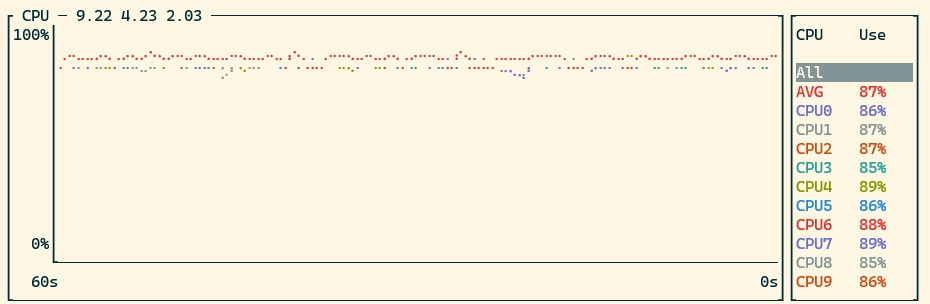
\includegraphics[alt={Graphique},width=\textwidth]{imgs/bottom-lifo.jpg}
  \caption{Utilisation ressources sur la \mone~avec \docref{desc:th_pile}}
  \label{fig:btm-lifo}
\end{figure}

\subsubsection{Sélection aléatoire de tâche}
\begin{description}
  \item[\bone] \hspace{1em}
        \begin{description}
          \item[\mone] Le programme a été lancé \textbf{100 fois}.
                Le temps moyen d'exécution a été de \textbf{0,390 secs}
          \item[\mtwo] Le programme a été lancé \textbf{100 fois}.
                Le temps moyen d'exécution a été de \textbf{0,438 secs}
        \end{description}

  \item[\btwo] \hspace{1em}
        \begin{description}
          \item[\mone] Le programme a été lancé \textbf{100 fois}.
                Le temps moyen d'exécution a été de \textbf{0,438 secs}
          \item[\mtwo] Le programme a été lancé \textbf{100 fois}.
                Le temps moyen d'exécution a été de \textbf{1,887 secs}
        \end{description}
\end{description}

Cette implémentation est identique à \docref{stats:stack}, à l'exception que
l'on récupère une tâche aléatoire de la pile au lieu d'y prendre la dernière
ajouté.

Cette façon de faire réduit les performances.

\subsection{Répartition par \ws}
\begin{description}
  \item[\bone] \hspace{1em}
        \begin{description}
          \item[\mone] Le programme a été lancé \textbf{100 fois}.
                Le temps moyen d'exécution a été de \textbf{0,229 secs}
          \item[\mtwo] Le programme a été lancé \textbf{100 fois}.
                Le temps moyen d'exécution a été de \textbf{0,308 secs}
        \end{description}

  \item[\btwo] \hspace{1em}
        \begin{description}
          \item[\mone] Le programme a été lancé \textbf{100 fois}.
                Le temps moyen d'exécution a été de \textbf{0,447 secs}
          \item[\mtwo] Le programme a été lancé \textbf{100 fois}.
                Le temps moyen d'exécution a été de \textbf{1,131 secs}
        \end{description}
\end{description}

Dans cet implémentation, on n'utilises plus une pile mais un deque de tâches.
Cette façon de faire est légèrement meilleur que \docref{desc:th_pile}.

Dans la \autoref{fig:btm-ws}, on observe que les \coeur{}s du CPU sont
proche de 100\% d'utilisation. Comparé à \docref{stats:stack}, on gagne
en moyenne \approx~10\% de l'utilisation du processeur dans son entièreté.

\begin{figure}[h!]
  \centering
  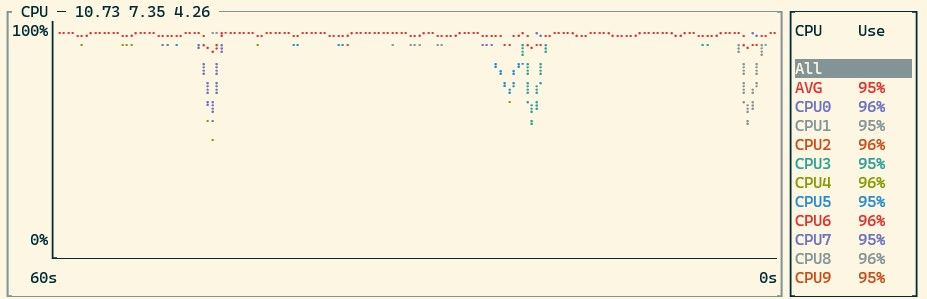
\includegraphics[alt={Graphique},width=\textwidth]{imgs/bottom-ws.jpg}
  \caption{Exploitation des ressources sur la \mone~avec \docref{desc:ws}}
  \label{fig:btm-ws}
\end{figure}

\clearpage
\appendix
\section{Crédits}

J'ai utilisé un bout de code de \href{https://expreg.org/amsi/C/}{Farès Belhadj}
d'un TP de L2 pour afficher une image au format \texttt{bmp} afin vérifier que
le \btwo~fonctionnait correctement. Ce qui donne la \autoref{fig:mandelbrot}.

\begin{figure}[h!]
  \centering
  
\includegraphics[alt={Fractale mandelbrot},width=0.7\textwidth]{imgs/mandelbrot.jpg}
  \caption{Example de Mandelbrot}
  \label{fig:mandelbrot}
\end{figure}

\end{document}
